\chapter{Discussion}
\label{Chap5}
Que conclure d'après les résultats?
\section{Powder ageing}
\subsection{Grain size and distribution}


\subsection{Composition}

\section{Density measures assessments}
\label{DDMA}
\subsection{Measures comparison}
%\subsection{Hydrostatic weighing}

Several methods were used to measure the densities of the specimens throughout this work: hydrodensimetry (both with and without preliminary polishing) and RODIA. The different techniques were performed on a few specimens in order to draw a comparison of the results and reach a deeper understanding of the methods reliability. The results are gathered on figures ....\\

One can expect the first option to reduce the risks of air trapping by the surface roughness during the underwater weighing, which can distort the results (by overestimating the closed porosities volume). %to observe potential inhomogeneous distributions of the closed porosities in the specimens.


\subsection{Relative optical density image analysis}
\label{DRODIA}

The estimation of the relative density through RODIA can be distorted on many grounds. First, the distribution of porosities is inhomogeneous on the analysed surface. Multiple photos must thus be taken with a systematic manner for each specimen to constitute a representative sample.\\

Second, the quality of the photographs has a critical role. The isolation of the porosities during the thresholding requires a substantial difference of pixel intensity between the holes and the material. Since some porosities and some zones of the material can appear respectively brighter or darker than was is expected, there are risks that one isolates spots and/or not actual porosities. Additionally, the thresholding is manual and thus prone to slight human errors. \\

Most importantly, the finite resolution of the camera implies that sufficiently small porosities are not visible on the pictures. 

One can expect the the density measurement through RODIA to be a biased method, due to the discretisation in pixels among other things. Results for pictures with different magnifications were compared to quantify these effects. For this purpose, a picture was taken under 5x magnification and two under 10x magnification. The former was delimited to match the visible zones on the latter (see figure \ref{fig:RODIA1}). The same two zones - named A and B - were thus analysed for different levels of resolution.\\

\begin{figure}[ht]
	\centering
	\centerline{\includegraphics[scale=0.075]{Images/RODIA1}}
	\decoRule
	\caption[50x magnification picture of specimen X200-180319-cub1 and delimitation of the zones A and B]{50x magnification picture of specimen X200-180319-cub1 and delimitation of the zones A and B}
	\label{fig:RODIA1}
\end{figure}

\begin{figure}[ht]
	\centering
	\centerline{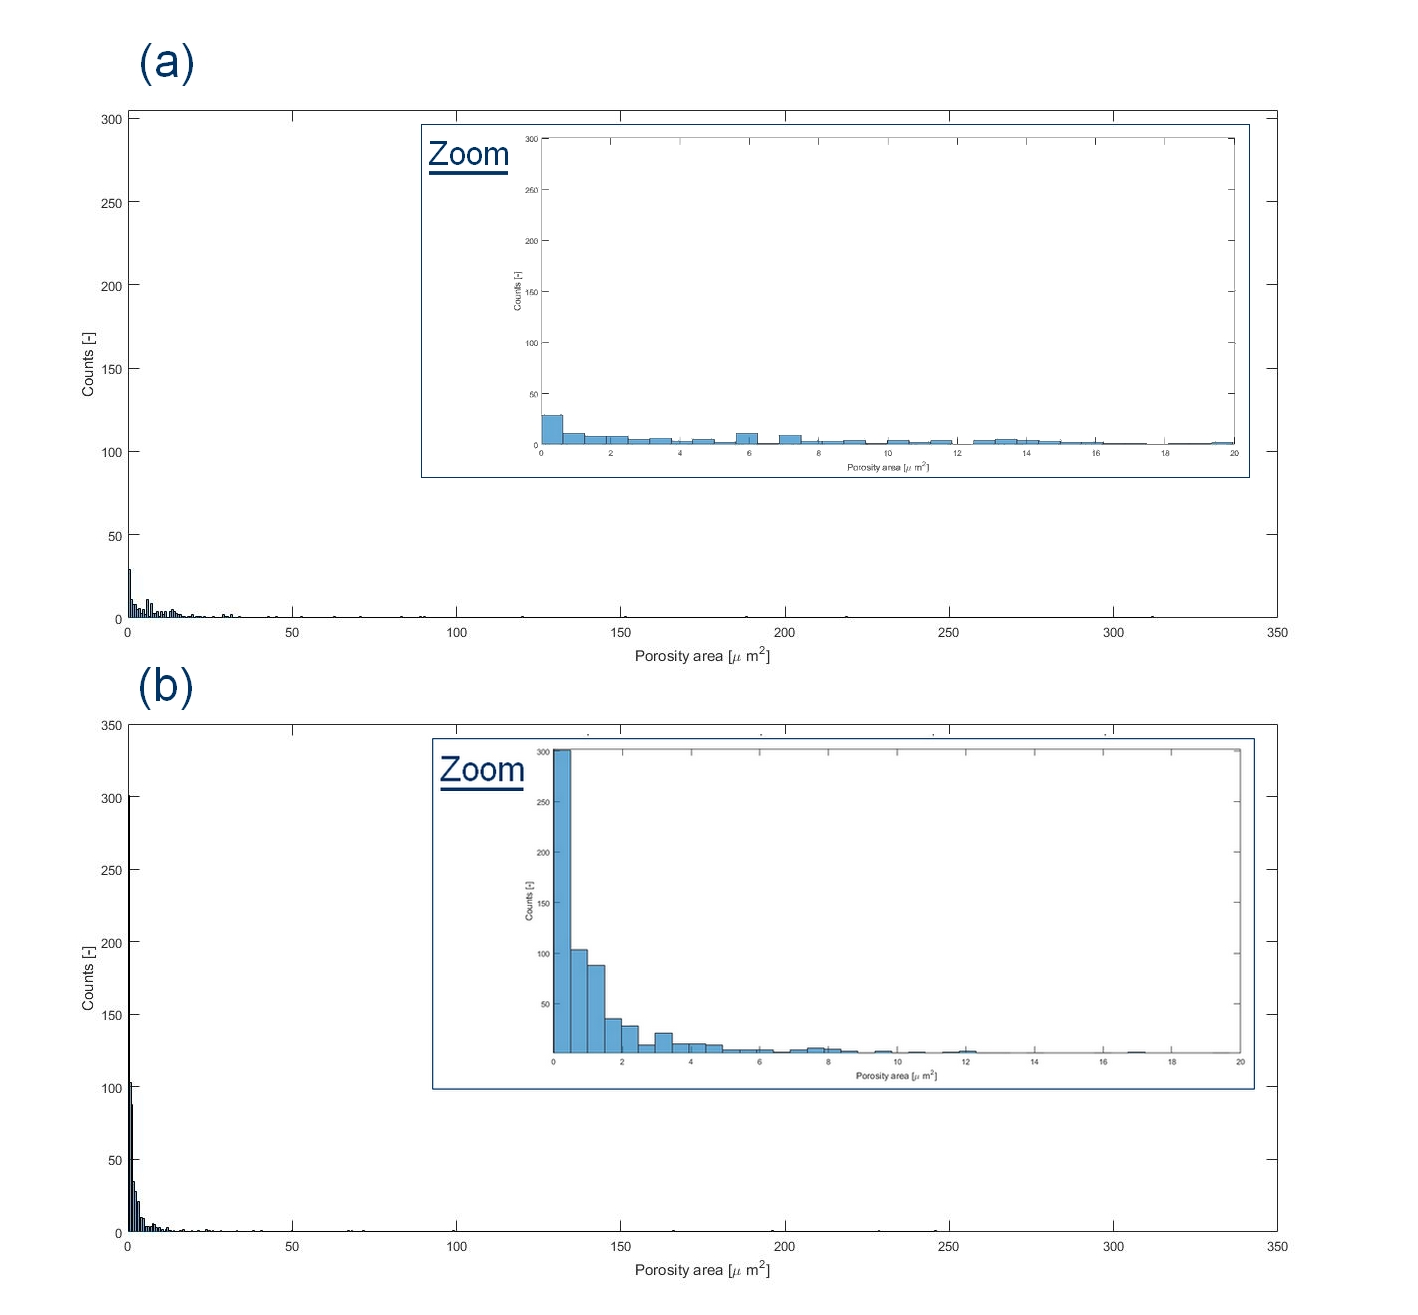
\includegraphics[scale=0.43]{Images/RODIAHist}}
	\decoRule
	\caption[Histograms of porosities areas occurrences from pictures of specimen X200-180319 on zone A under (a) 50x magnification (b) 100x magnification]{Histograms of porosities areas occurrences from pictures of specimen X200-180319 on zone A under (a) 50x magnification (b) 100x magnification. Truncation along the x axis. }
	\label{fig:RODIAH}
\end{figure}


The comparison of figures \ref{fig:RODIA2} (b) and (d) shows that much more small porosities are isolated if the resolution is refined. This is confirmed by the histograms on figure \ref{fig:RODIAH}. The threshold of porosity area for detection in the case of 5x magnification is 7.84 [$\mu m^2$] whereas it is 1.96 [$\mu m^2$] for 10x magnification. This area corresponds to a pixel in each case. It is also worth noting that there is an overall tendency to overestimate the areas at lower resolution, which counterbalances slightly the low number of detected porosities. \\

\begin{figure}[ht]
	\centering
	\centerline{\includegraphics[scale=0.44]{Images/RODIA2}}
	\decoRule
	\caption[Zone A of specimen X200-180319-cub1: (a) Delimitation from original picture under 50x magnification (b) Porosities isolation from 50x magnification picture (c) Original picture under 100x magnification (d) Porosities isolation of 100x magnification picture]{Zone A of specimen X200-180319-cub1: (a) Delimitation from original picture under 50x magnification (b) Porosities isolation from 50x magnification picture (c) Original picture under 100x magnification (d) Porosities isolation of 100x magnification picture}
	\label{fig:RODIA2}
\end{figure}


The RODIA results for zones A and B are outlined in table \ref{tab:RODIASS}. It was observed that pictures with lower resolution have the tendency to lead to the overestimation of the relative density. The order of magnitude of the difference is of few hundredths of percent. The method is thus presumably positively biased. However, the observed effect is minor: this is probably due to the fact that the undetected porosities are the smallest, which influence the less the calculated density value.\\

\begin{center}
	\begin{table}[ht]
		\centerline{\begin{tabular}{|c|c|c|}
				\hline
				Zone & Magnification & Measured relative density [$\%$] \\
				\hline
				A & 50x  & 99.87\\
				A & 100x & 99.84\\
				B & 50x & 99.86\\
				B & 100x & 99.85\\
				\hline
		\end{tabular}}
		\caption[RODIA results for zones A and B of specimen X200-180317 with 50x and 100x magnification]{RODIA results for zones A and B of specimen X200-180317 with 50x and 100x magnification}
		\label{tab:RODIASS}
	\end{table}
\end{center}

Taking pictures at refined magnification could be considered to better the precision of the method. This would, however, require to augment the number of analysed pictures to have a sample of pictures as representative. A picture with doubled magnification covers indeed four times less surface. The number of analyses should thus be quadrupled to take as much information into account.\\

[PARLER AUSSI DE L'APPROX de FRACTION SURFACIQUE DES PORES = A LA VOLUMIQUE]

\section{Density and hardness study}

\subsection{Parameters optimisation}

\subsection{Reproducibility}

\section{Characterisation of the as-built samples}

\subsection{Melt pools sizes and distribution}

\subsection{Microstructure}

\subsection{Residual stresses}

\subsection{Mechanical properties}

\section{Characterisation of the heat treated samples}

\subsection{Heating process}
Quand on chauffe à 300 deg, on chauffe déjà longtemps à plus de 200 deg

\subsection{Microstructure}

\subsection{Residual stresses}

While the usual stress-relief treatment for aluminium alloys -to hours holding at 300$^\circ$ C- does indeed relieve stresses inside the specimen, it also triggers significantly the diffusion of alloying elements, altering the material microstructure.

\subsection{Mechanical properties}


\subsection{Optimisation}



%\section{Mechanical testing}